

%----------------------------------------------------------------------------------------
%	PACKAGES AND OTHER DOCUMENT CONFIGURATIONS
%----------------------------------------------------------------------------------------

\documentclass[12pt, twoside]{book} % 12 pt font, two-sided book style
\usepackage[a4paper, includehead, headheight=0.6cm, inner=3cm ,outer=2.5cm, top=2.5 cm, bottom=2.5cm]{geometry}  % Changing size of document
\usepackage[english]{babel} % The document is in English
\usepackage[utf8]{inputenc} % UTF8 encoding
\usepackage[T1]{fontenc} % Font encoding
\usepackage{csquotes}

\usepackage{graphicx} % For including images
\graphicspath{{./fig/}} % Specifies the directory where pictures are stored

\usepackage{longtable} % tables that can span several pages
\usepackage{fancyhdr} % For the headers
\usepackage[font=footnotesize,bf]{caption}%FIG in bold
\usepackage{subcaption}

\usepackage{float,placeins} % Force table Here
\usepackage{booktabs}

\newcommand{\numberedchapter}{ % Preparation for numbered chapters
	\cleardoublepage % To make sure the previous headers are passed
	\fancyhead[RE]{{\bfseries \leftmark}}% Headers for left pages
	\fancyhead[LO]{{\bfseries \rightmark}}}% Headers for right pages
\newcommand{\unnumberedchapter}[1]{ % Preparation for unnumbered chapters
	\cleardoublepage % To make sure the previous headers are passed
	\addcontentsline{toc}{chapter}{#1} % Also adds the chapter name to the Contents
	\fancyhead[RE]{{\bfseries #1}} % Headers for left pages
	\fancyhead[LO]{}}%Headers for right pages

% special font for chapter

\usepackage[scaled=.90]{helvet}% Helvetica, served as a model for arial
\usepackage[dvipsnames*,svgnames]{xcolor}
\usepackage{titlesec}
\titleformat{\chapter}[display]
  {\normalfont\sffamily\huge\bfseries\color{FireBrick}}
  {\chaptertitlename\ \thechapter}{20pt}{\Huge}
\titleformat{\section}
  {\normalfont\sffamily\Large\bfseries\color{SteelBlue}}
  {\thesection}{1em}{}


\usepackage{emptypage} % No headers on an empty page

%\usepackage{eso-pic} % For the background picture on the title page
%\newcommand\BackgroundPic{%
%\put(-250,-160){%
%\parbox[b][\paperheight]{\paperwidth}{%
%\vfill
%\centering
%\includegraphics[width=\paperwidth]{symbol.jpg}%
%\vfill
%}}}

\usepackage{hyperref} % Adds clickable links at references
\usepackage{fourier}

%----------------------------------------------------------------------------------------
%	ADD YOUR CUSTOM VALUES, COMMANDS AND PACKAGES
%----------------------------------------------------------------------------------------

% Open Preamble/mydefinitions.tex and enter some values (name, thesis title...) 
% and include your own custom LaTeX functions and packages

\DeclareUnicodeCharacter{0301}{*************************************}

%----------------------------------------------------------------------------------------
%	VALUES FOR THE THESIS
%----------------------------------------------------------------------------------------

\newcommand{\name}{Muhammad Mun'im Ahmad Zabidi (WVA170038)} % Author name
\newcommand{\thesistitle}{Edge Computing with Deep Learning for Bird Recognition} % Title of the thesis
\newcommand{\submissiondate}{January, 2020} % Submission date "Month, year"
\newcommand{\supervisor}{Dr. Rohana binti Mahmud} % Supervisor name
\newcommand{\cosupervisor}{P.M. Dr. Muhammad Yamani Idna bin Idris} % Co-Supervisor name, comment this line if there is none

\usepackage[backend=biber, 
sorting=none,
%citestyle=authoryear,
%maxnames=1,
url=false,natbib=true, isbn=false,
]{biblatex}
\bibliography{references}

%----------------------------------------------------------------------------------------
%	BIBLIOGRAPHY STYLE (pick the style you want)
%----------------------------------------------------------------------------------------

%\usepackage[square, numbers, sort&compress]{natbib} % for bibliography - Square brackets, citing references with numbers, citations sorted by appearance in the text and compressed (as in [4-7])
%\usepackage[longnamesfirst,round]{natbib} % Natural Sciences bibliography

%\bibliographystyle{Preamble/physics_bibstyle} % You may use a different style adapted to your field
%\bibliographystyle{unsrtnat} % You may use a different style adapted to your field


%----------------------------------------------------------------------------------------
%	YOUR PACKAGES (be careful of package interaction)
%----------------------------------------------------------------------------------------

\usepackage{amsthm,amsmath,amssymb,amsfonts,bbm}% Math symbols

%----------------------------------------------------------------------------------------
%	YOUR DEFINITIONS AND COMMANDS
%----------------------------------------------------------------------------------------

% New Commands
\newcommand{\bea}{\begin{eqnarray}} % Shortcut for equation arrays
\newcommand{\eea}{\end{eqnarray}}
\newcommand{\e}[1]{\times 10^{#1}}  % Powers of 10 notation

% Defining a theorem box for Criteria
\newtheorem{critere}{Criterion}
\newcommand{\crit}[2]{
\begin{center}  
\fbox{ \begin{minipage}[c]{0.9 \textwidth}
\begin{critere}
\textbf{\textup{ #1}} --- #2
\end{critere}
\end{minipage}  } \end{center}
}

\begin{document}

%----------------------------------------------------------------------------------------
%	TITLE PAGE
%----------------------------------------------------------------------------------------

\pagestyle{empty} % No page numbers
\frontmatter % Use roman page numbering style (i, ii, iii, iv...) for the preamble pages

\begin{titlepage}
%\AddToShipoutPicture*{\BackgroundPic}
\begin{center}
\vfill

\includegraphics[width=.5\textwidth]{um}
\vfill
%{\large \scshape Universiti Malaya}\\[1.4cm]
{\Large PhD Thesis Proposal}\\[0.5cm]
\rule{\textwidth}{1.5pt}\\[0cm]
{\huge \bfseries \sffamily \thesistitle \par \ }\\[-0.5cm]
\rule{\textwidth}{1.5pt}\\[2.5cm]
\hfill  \textit{by}\\[1cm]
\hfill  {\large \bfseries\name}\\
\vfill
\hfill  \textit{Supervisors}\\[.8cm]
{\hfill \large  \textbf{\supervisor}} \\ [.5cm]
\ifx\cosupervisor\undefined\else{\hfill \large  \textbf{\cosupervisor}} \\ \fi
\vspace{1cm}
\hfill  \submissiondate
\end{center}
\end{titlepage}

%----------------------------------------------------------------------------------------
%	PREAMBLE PAGES (comment out unnecessary pages)
%----------------------------------------------------------------------------------------

\pagestyle{fancy} % Changes the headers
\renewcommand{\chaptermark}[1]{ \markboth{#1}{}} % Getting the chapter name right
\renewcommand{\sectionmark}[1]{\markright{\thesection\; #1}} % Getting the section name right
\fancyhf{}% Clears header and footer
\fancyhead[RO,LE]{\thepage} % page number on the outside of headers

\unnumberedchapter{Abstract} 
\chapter*{Abstract} 
%\subsection*{\thesistitle}


Birds are important indicators of the health of the environment. Birds pollinate plants, disperse plant seeds and suppress pest populations. Accurate bird recognition helps to quantify the effects of human activity on avian biodiversity. Most researchers use passive acoustic monitors (PAMs) to collect recordings spanning hundreds of hours resulting in large volumes of data. Due to the size of recordings, bird identification remains an almost impossible task to be done manually. As PAMs could be remotely located, the sound files may require substantial effort to collect.

The edge computing paradigm allows data processing tasks to be performed at the edge of the network. This new approach reduces system running time, memory requirements and energy consumption for a wide range of big data applications. Combined with long-range low-power radio networks, applying the approach for bird recognition should reduce the need to manually retrieve sound recordings which contain mostly redundant information anyway.

Bird sound recognition applies many of the same techniques as sound event detection and keyword spotting (KWS). For large scale bird recognition, the highest accuracies are currently achieved using ImageNet-class convolutional neural networks (CNNs). These large CNNs are computationally complex in terms of multiply-and-add operations and require a lot of memory. For edge computing, as an alternative is required to preserve battery life and reduce systems costs.

This research aims to identify and propose suitable low-complexity algorithms for bird sound detection and classification. The approach to apply the two-stage cascade architecture used in KWS \cite{Sigtia2018}. The first stage is the bird detector. It is a binary classifier that detects a bird sound of any kind. In a battery-powered device, the first stage is always turned on, therefore, performs minimal computations to reduce energy usage. The detector stage is to be constructed using a binarized convolutional network (BNN). The second stage is the bird classifier. The output of the classifier is the identified bird species. This stage requires more computational effort as it consists of an integer CNN. In a battery-power device, the second stage is turned on only when the first stage detects a bird sound to reduce energy consumption and improve recognition accuracy. In addition to exploring several BNN and CNN configuration, the research will investigate the impact of various audio features on recognition accuracy.

Preliminary works have been to collect sound files for 10 species of birds and to test the recognition accuracy on the ResNet-50 CNN using short-time Fourier transform (STFT) and Mel Frequency Cepstrum Coefficients (MFCC) features. %For the remainder of the research, 10 more species of birds will be added.
 Alternative CNN configurations and audio features will be explored. The accuracy and complexity of the proposed algorithms will be benchmarked against state-of-the-art results.

%----------------------------------------------------------------------------------------
%	LIST OF CONTENTS/FIGURES/TABLES
%----------------------------------------------------------------------------------------

\unnumberedchapter{Contents}
\tableofcontents % Write out the Table of Contents

\unnumberedchapter{List of Abbreviations}
\chapter*{List of Abbreviations}
\thispagestyle{empty}

\vspace{0.5cm}

\begin{longtable}{|c|l|} 
 \hline
  \textbf{Abbreviation} & \textbf{Definition} \\ \hline
    AOP & Always-On Processor \\ \hline
    ASIC & Applcation-Specific Integrated Circuit \\ \hline
    BNN & Binarized Neural Network \\ \hline
    c-MAP & classification Mean Average Precision \\ \hline
    CNN & Convolutional Neural Network \\ \hline
    CQT & Constant-Q Transform \\ \hline
    DFT & Discrete Fourier Transform \\ \hline
    DSP & Digital Signal Processing \\ \hline
    FFT & Fast Fourier Transform \\ \hline
    GPU & Graphical Processing Unit \\ \hline
    IoT & Internet-of-Things \\ \hline
    IPS & Inferences per second \\ \hline
    KWS & Keyword Spotting \\ \hline
    MAC & Multiply-Accumulate \\ \hline
    mAP & mean Average Precision \\ \hline
    ML & machine learning \\ \hline
    MFCC & Mel-Frequency Cepstral Coefficients \\ \hline
    PAM & Passive Acoustic Monitor \\ \hline
    ReLu & Rectified Linear Unit \\ \hline
    SIF & Spectrogram Image Features \\ \hline
    SoC & System-on-Chip \\ \hline
    STFT & Short-Time Frequency Transform \\ \hline
    TN & True Negative \\ \hline
    TP & True Positive \\ \hline
    VAD & Voice Activity Detector \\ \hline
\end{longtable} % Import your chapters here


%----------------------------------------------------------------------------------------
%	THESIS MAIN TEXT - CHAPTERS
%----------------------------------------------------------------------------------------

\addtocontents{toc}{\vspace{2em}} % Add a gap in the Contents, for aesthetics
\mainmatter % Begin numeric (1,2,3...) page numbering

\numberedchapter
\chapter{Introduction}

\section{Background}



Sound event recognition is a growing area of research with in recent years.
Automatic recognition of sound events is useful in many applications including audio surveillance (\cite{Foggia2015}), multimedia retrieval (\cite{Wold1996}), animal monitoring \citep{Mcloughlin2019} and environmental sound monitoring (\cite{Chu2009}).
Bird recognition by acoustic means is one of the interesting sub-areas of sound event recognition.

The rate of biodiversity loss and ecological degradation is unprecedented. 
Birds play an important role in the ecosystem as they disperse plant seeds, pollinate plants, and subdue pest populations and birds are good indicators of the health of the environment \citep{Priyadarshani2018}.
The use of sounds for monitoring of bird species offers an effective approach as most birds use vocalisations as their primary communication method (\cite{Gregory2010}).
%Birds are good subjects for bioacoustic census methods since most of the species use vocalizations to attract mates and to advertise territories (\cite{Gaunt2004})

Acoustic analysis of birds is challenging. Most people can recognize at most only a few birds and there are over nine thousand bird species in the world.
Most researchers use passive acoustic monitors (PAMs) left on site to collect recordings spanning hundreds of hours resulting in large volumes of data \citep{Sugai2019}. 
PAMs provide many benefits over the use of field observers, such as collecting data at large spatial area and different times of day or year (\cite{Digby2013}).
Due the overwhelming amount of data, bird identification remains an almost impossible task to be done manually.
Therefore, automating the process of bird identification is important.
Another issue is that as PAMs could be remotely located, retrieving the recorded sound files may require substantial effort and impose delays of days or weeks after the actually recording.

%Acoustic sensors left on site can continuously capture the acoustic activity and as 
%The greatest challenge with automated recordings though is to find the sounds of bird species of interest within these extensively long recordings

The edge computing and Internet-of-Things (IoT) paradigms allow data processing tasks to be performed at the edge of the network, close to the point of data acquisition.
This new approach reduces system running time, memory requirements and energy consumption for a wide range of big data applications.
Combined with long-range low-power radio networks, applying the approach for bird recognition should reduce the need to manually retrieve sound recordings which contain mostly redundant information anyway.


Bird sound recognition applies many of the same techniques as sound event detection and keyword spotting (KWS).
For large scale bird recognition, the highest accuracies are currently achieved using ImageNet-class convolutional neural networks (CNNs) \citep{Kahl2019}.
These large CNNs are computationally complex in terms of multiply-and-add operations and require a lot of memory.
For edge computing, as an alternative is required to preserve battery life and reduce systems costs.

This research aims to identify and propose suitable low-complexity algorithms for bird sound detection and classification.
The approach to apply the two-stage cascade architecture used in KWS (\cite{Sigtia2018}).
The first stage is the bird detector.
It is a binary classifier that detects a bird sound of any kind. 
In a battery-powered device, the first stage is always turned on, therefore, performs minimal computations to reduce energy usage.
The detector stage is to be constructed using a binarized convolutional network (BNN). The second stage is the bird classifier.
The output of the classifier is the identified bird species.
This stage requires more computational effort as it consists of an integer CNN.
In a battery-powered device, the second stage is turned on only when the first stage detects a bird sound to reduce energy consumption and improve recognition accuracy.
In addition to exploring several BNN and CNN configuration, the research will investigate the impact of various audio features on recognition accuracy.


\section{Research Questions}

Some	 of	 the	major	 questions	 that	 are	 addressed	 in	 audio recognition:

\begin{itemize}
\item	 “If	 waveforms	 are	 processed,	 what	 techniques	 can	 be	 adopted	for	signal	processing?”
\item	“If	spectrograms	are	processed,	what	 techniques	can	be	
adopted	for	time-frequency	domain?”
\item	“What	are	the	useful	acoustic	components	for	animal	call	
recognition?”
\item Are features such as MFCC, frame power effective for classification
\item	 “How	 can	 the	 developed	 species	 recognition	 system	 be	 evaluated?”
\end{itemize}



\section{Problem Statement}
 % Import your chapters here


\chapter{Literature Review}

This chapter establishes the context of the research. First, methods for bird recognition are introduced. 
Then, the application of deep learning for bird recognition are elaborated.
The use of edge computing in sound event detection are discussed next.
Finally, gaps in the application of edge computing and deep learning for bird recognition are clarified.

\section{Bird Recognition}

%\begin{figure}
%\centering
%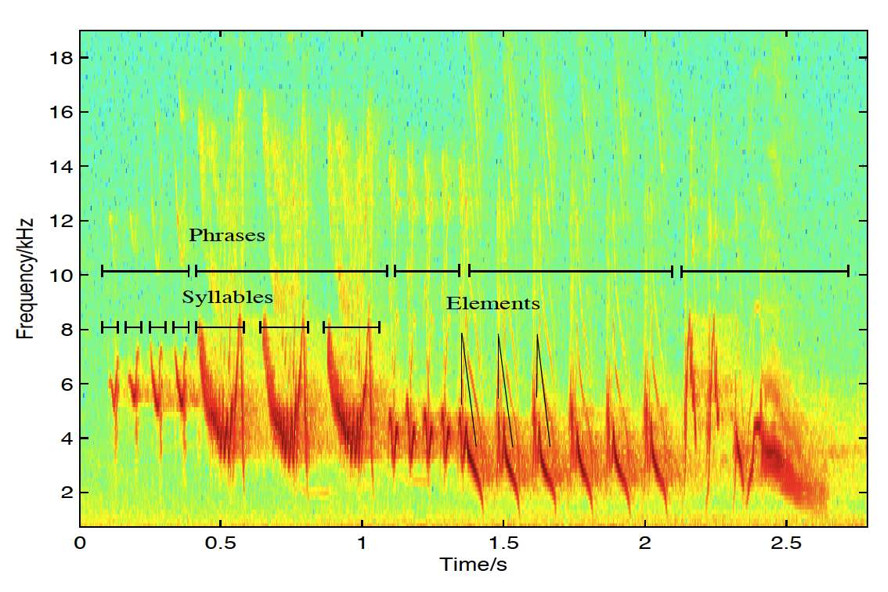
\includegraphics[scale=.33]{birdspectrogram}
%\caption{Comparison of human and bird sound generation.}
%\end{figure}

Birds are important indicators of the health of the environment. 
The traditional method of bird monitoring is by point counts where an observer records all birds seen and heard at a fixed location \cite{Shonfield2017}.
Since birds are easily detected by sound, using bird recognition based on acoustic signals can augment or even supplant the point count method \citep{Kuaga2019}.

Passive acoustic monitors (PAMs) also known as autonomous recording units (ARUs) left on site can continuously capture audio recordings and offer many advantages over field observers \citep{Digby2013,Sugai2019}.
The sounds are processed through spectrogram reading and/or listening by experienced observers.
Due to sheer volume of data, it is not feasible to manually process weeks' or months’ worth of recordings.
The trend today is towards automatic recognition \citep{Aide2013}.

Bird vocalizations can be classified as songs and calls. Songs attract mates and advertise territories during the breeding season in songbirds. Calls are used during foraging, social and antipredator communications. Songs and calls can differ substantially in time and frequency components \cite{Velez2015}.

\begin{figure}%[h]
\centering
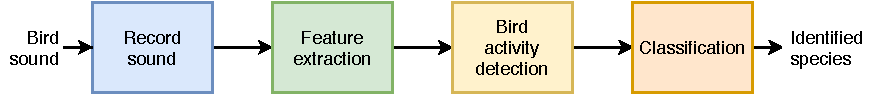
\includegraphics[scale=1]{birdrecognitionmodules}
\caption{Modules for bird species recognition.}
\label{birdrecognitionmodules}
\end{figure}

A typical workflow for identifying birds by sound is shown in Fig. \ref{birdrecognitionmodules}.
The first module records bird sounds into \textit{wav} format and divides the sound into fixed length frames.
A feature vector is generated from each frame for the next module. Next, the bird activity detector selects only frames which contain bird vocalizations to be passed on the classification stage. The other parts of the sound are discarded. This stage increases classification accuracy \cite{Stastny2018}. Finally the classification stage identifies the bird species.

%The remainder of this section compares classifiers used for bird recognition task. Finally, the various features can be extracted from sound, focusing on time-frequency image-based representation.


\subsection{Classifiers}

Bird detection is such an interesting challenge that several competitions are held regularly to find the best classifier algorithm. 
One such competition is BirdCLEF, held annually by the Conference and Labs of the Evaluation Forum (CLEF). 
Table \ref{birdclefwinners} lists the winners since 2015.
Since 2016, all winners have been using classifiers based on convolutional neural networks (CNNs).
Outside of BirdCLEF, other researchers have also found CNN to consistently outperform other classifiers in most use cases.

\begin{table}[h]
\renewcommand{\arraystretch}{.75}
\caption{BirdCLEF winners post-2015. MAP and c-mAP use different methodologies to compute.}
\label{birdclefwinners}
\centering
\
\begin{tabular}{clcc}
\toprule
\textbf{Year} & \textbf{Method}	&  \textbf{Accuracy} & \textbf{Reference} \\
\midrule
2015 & Decision tree & mAP = 0.454 & \cite{Goeau2015} \\
2016 & 5-layer CNN & mAP = 0.555 & \cite{Goeau2016}\\
2017 & Inception v4 CNN & c-mAP = 0.182 & \cite{Sevilla2017}\\
2018 & Inception v3 CNN & c-mAP = 0.193 & \cite{Goeau2018} \\
2019 & Inception v3 and ResNet CNN & c-mAP = 0.356 & \cite{Kahl2019} \\
\bottomrule
\end{tabular}
\end{table}

Due to the clear advantage of CNN, this proposal will proceed with the discussion of CNN and its application to sound event detection.

\subsection{Features}

CNN works on two-dimensional images.
Bird sounds are one-dimensional signal representations.
Sounds are commonly converted to two-dimensional representations or spectrograms before any processing by CNN.
This section discusses spectrograms and its variations.

\subsubsection{Spectrogram}

A spectrogram in an image produced by applying the discrete Fourier transform (DFT) to a windowed signal.
The Short-Time Fourier Transform (STFT) computes the frequency and phase contents of a signal over time. 
The Fourier transform of a signal is taken by multiplying a window function for a short period of time:

\[
\mathrm{STFT}\{x(t)\}(\tau,\omega) \equiv X(\tau,\omega) = \int^\infty_\infty x(t)\omega(t-\tau)e^{-i\omega t}dt
\]

\noindent
where $\omega(\tau)$ is the window function, commonly a Hamming or Hanning windows centered around zero, and $x(t)$ is the signal to be transformed.

In the discrete version of STFT, the data to be transformed is split into frames. Frames usually overlap to reduce the effects of windowing. Mathematically, it is:

\[
\mathrm{STFT}\{x[n]\}(m,\omega) \equiv X(m,\omega) = \sum^\infty_{n=-\infty} x[n]\omega[n-m]e^{-j\omega t}dt
\]

\noindent
where $x[n]$ is the signal, and $\omega[n]$ is the window. Discrete-time STFT is typically performed on computer using optimized routines called the Fast Fourier Transform (FFT). Fig. \ref{koel} shows the time representation and spectrogram equivalent of an Asial koel.




\begin{figure}[H]
     \centering
     \begin{subfigure}[b]{0.47\textwidth}
         \centering
         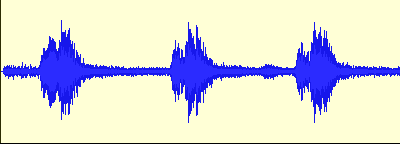
\includegraphics[width=\textwidth]{koel-wav}
         \caption{Time representation.}
 %        \label{fig:y equals x}
     \end{subfigure}
     \hfill
     \begin{subfigure}[b]{0.47\textwidth}
         \centering
         
\includegraphics[width=\textwidth]{koel-spec}
         \caption{Spectrogram.}
%         \label{fig:three sin x}
     \end{subfigure}
    \caption{Asian koel bird call in time and frequency representations.}
    \label{koel}
\end{figure}



\subsubsection{Mel-Frequency Cepstral Coefficients (MFCC)}

Humans do not perceive frequency in a linear manner because the ears becomes less selective as frequency increase above 1 kHz. The Mel scale was developed to compensate for this.
MFCC works well with human voice and to a major extent on bird sounds because the sound production mechanisms of human and birds have some similarities. The approximate expression for the Mel scale is:

\[
F_\mathrm{mel} = \frac{1000}{log(2)} \cdot \left[1+\frac{F_\mathrm{Hz}}{1000}\right]
\]


\begin{figure}[h]
    \centering
    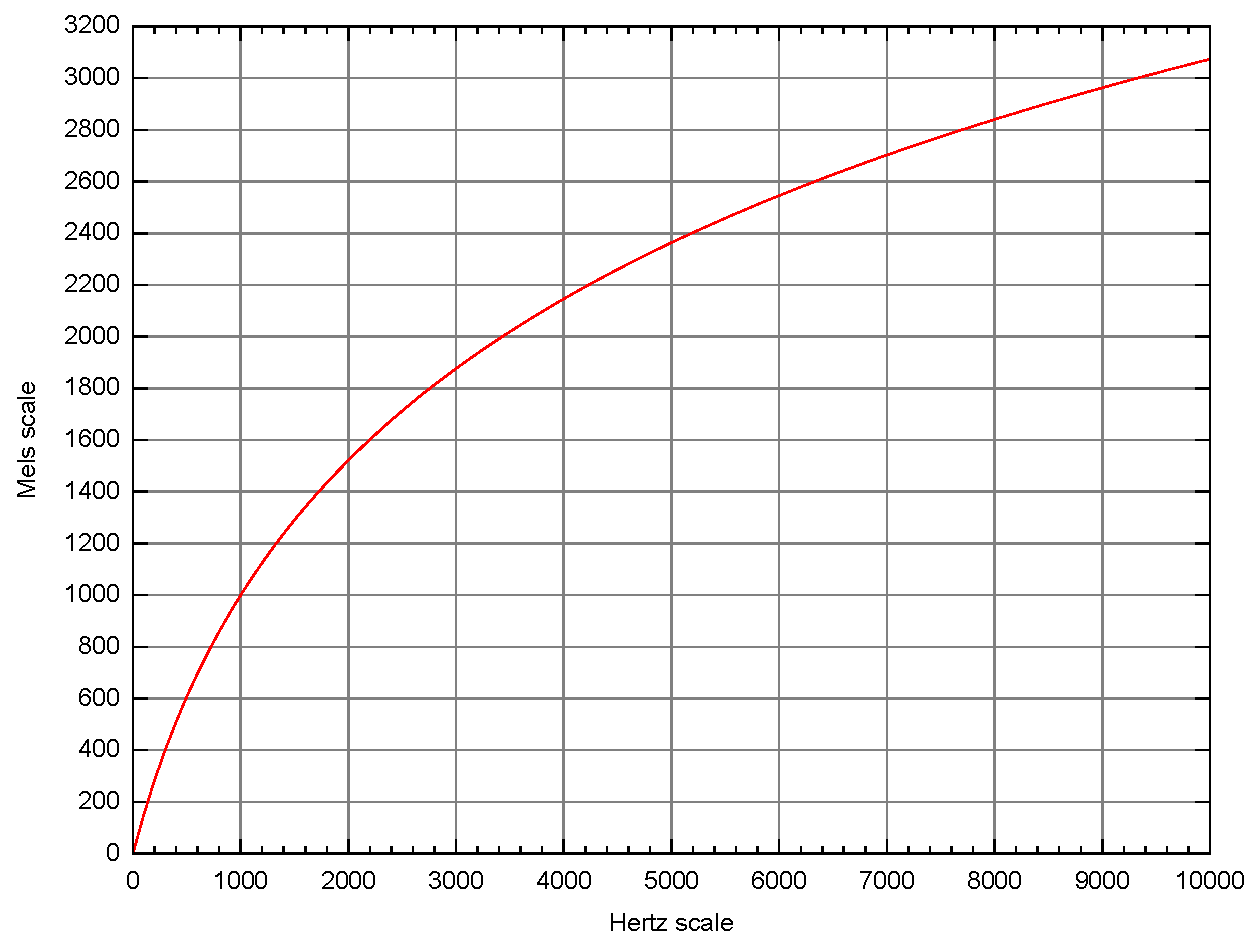
\includegraphics[width=.5\textwidth]{mel-hz-plot}
    \caption{Mel-Hz plot.}
    \label{mel-hz-plot}
\end{figure}

\begin{figure}[h]
    \centering
    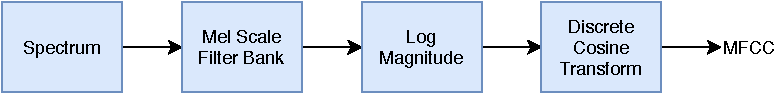
\includegraphics[width=.8\textwidth]{mfcc}
    \caption{Computation of MFCC.}
    \label{mfcc}
\end{figure}

The relationship between Mel scale and linear frequency  is illustrated in Fig. \ref{mel-hz-plot}.
For each frame of speech signal, a MFCC vector is computed as illustrated in Fig. \ref{mfcc}. The spectrum is passed through the Mel filter bank. Then the logarithm of the filter bank output is transformed by applying the discrete cosine transform (DCT). DCT decorrelates the extracted features facilitating the extraction of salient features. Typically MFCC is represented by the first 13 coefficients of the Mel cepstrum.


\subsubsection{Mel Spectrogram}

The mel spectrogram are computed similar to MFCC but without computing the discrete cosine transform. For some applications, the mel spectrogram produced results comparable to MFCC \cite{Lasseck2018}.

\subsubsection{Cochleagram}

Gammatone is another filter inspired by human hearing. The filter bank simulates the cochlea, and the produced spectrum is sometimes called the cochleagram \cite{Xie2017}. The Gammatone Frequency cepstral coefficients (GFCC) are computed as in Fig. \ref{gfcc}.

\begin{figure}[h]
    \centering
    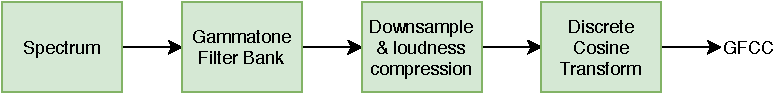
\includegraphics[width=.8\textwidth]{gfcc}
    \caption{Computation of GFCC.}
    \label{gfcc}
\end{figure}

The spectrum is passed through the Gammatone filter bank. Then loudness compression and DCT are applied. GFCCs are the first 22 feature extracted.

\subsubsection{Spectrogram Image Features (SIF)}

In spectrogram image features (SIF), features are extracted from the visual signature of the spectrogram. Taking advantage of the fact that spectrograms appear as recognisable images to humans, a spectrogram is mapped into several images with different dynamic ranges. The separate images are again partitioned into $9 \times 9$ blocks, and image moments are computed for each block. This method is robust to noise \cite{Dennis2010}. SIF is not applicable to CNNs as the the features extracted from spectrograms are used for classifications and the features no longer look like images expected by CNNs.

%Detect the bird vocalizations using \cite{Fodor2013}, \cite{Lasseck2015} and \cite{Potamitis2015}.

Other features that are commonly used with bird sounds include constant-Q transform (CQT), LPCC, fundamental frequency, zero crossing rate, spectral flux, spectral centroid and spectral flatness.


%\newpage
%-----------------------------------------------------------
% Section 2.2
%-----------------------------------------------------------

\section{Convolutional Neural Networks}

Convolutional Neural Network (CNN) -- also called ConvNets or CNNs -- are popular because they work well in difficult tasks such as image classification and object detection.

\subsection{Elements of CNN}

A typical CNN is illustrated in Fig. \ref{typicalcnn}. The three types of layers in convolutional neural network are convolution layer, pooling layer and fully connected layer.

\begin{figure}[H]
\centering
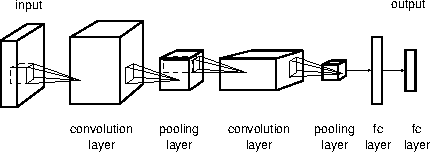
\includegraphics[scale=1.33]{typicalcnn}
\caption{An example CNN with two convolution
layers, two pooling layers and two fully-connected (FC) layers.
Cubes are 3-D tensors and rectangular shapes are 1-D tensors,
and the relative tensor size presents actual data volume \cite{Chen2016}.}
\label{typicalcnn}
\end{figure}

%Chen2016

\subsubsection*{Convolution Layer}

A convolution layer transforms the input image in order to extract features from it.
The input image is convolved with a kernel (or filter).
The two-dimensional output array from this operation is the output feature map.

A kernel is a small matrix which slides across the height and width of the  input image.
The dot product of the kernel and the image are computed at every spatial position producing the feature map.
The length by which the kernel slides is known as the stride length.

Color images have multiple channels, namely red, green, and blue, often referred to as the depth of the image.
A single color image is processed as three images by a convolutional layer.
Separate kernels are applied for each channel and the size of all the kernels must be the same.
The the output feature maps are stacked one after the other to create an output so that the number of channels is equal to the number of filters used. 

Finally to make up a convolution layer, a bias is added and an activation function is applied to increase the non-linearity in the output.
Traditionally, hyperbolic tangent or logistic sigmoid have been used. Today,  the rectified linear unit (ReLU) is more common as it computes faster while retaining sufficient discriminatory properties.

\subsubsection*{Pooling Layer}

Pooling layer is used to reduce the size of the representations and to speed up calculations, as well as to make some of the features it detects a bit more robust.
Typically pooling operations are maximum pooling and average pooling.
Maximum pooling extracts the maximum of a given kernel. 
On the other hand, average pooling computes the average of given kernel instead.

\subsubsection*{Fully-Connected Layer}

A fully-connected (FC) or dense layer integrates mid-level features at different spatial locations into a high-level representation, and at the same time, the last fully-connected layer is the classifier to rank the possibility of each class.

A fully-connected layer fuses locally extracted features from convolution layers into a high-level representative, and fully-connected layer utilizes a linear projection approach to map high-dimension feature vector to dense but low-dimension feature vector.

\subsection{CNN Complexity}

Calculating the number of parameters and operations enables different CNNs to compared in terms of computational complexity. This in turn enables the estimation of energy required for each inference.

A convolutional layer has these parameters: $C$, $Y$ and $X$  are channel, height and width of the input image, $H$ and $W$ are height and width of one kernel, and $N$, $Y'$ and $X'$ are channel, height and width of the output feature map.
The number of features to learn is $N\times C \times H \times W$.
The number additions required is then $(C\times H\times W-1)\times N\times Y'\times X'$ and the number of multiplications is $(C\times H\times W)\times N\times Y'\times X'$.

%For each feature map, a bias is added. Therefore, the total number of parameters is $(n\times m\times l+1)\times k$.

The size of the output feature map of a convolutional layer is found by $\mathit{input\_size}-(\mathit{filter\_size}-1)$. Normally padding is added to match the sizes, so that the expression becomes $\mathit{input\_size}+2\times \mathit{padding\_size}- (\mathit{filter\_size}-1)$.

The pooling layers has no parameters to learn. Its function is to reduce the image dimension.

In the fully-connected layer, all inputs has a trainable weight from each output of the previous layer. Therefore, for $M$ inputs and $N$ outputs, number of parameters and number of multiplications is $M\times N$. The number of additions is $(M - 1)\times N$ as we only need $n-1$ operations to add $n$ numbers.
The same calculation applies to the output layer as the output layer is fully-connected.

Table \ref{tabops} summarizes the number of operations and parameters required by different layer types.

\begin{table}[H]
\small
\centering
\caption{Number of operations of different layer type \cite{Chen2016}.}
\label{tabops}
\begin{tabular}{cccc}
\toprule
\textbf{Layer type}	&	\textbf{Additions} &	\textbf{Multiplications} & \textbf{Weight Size} \\
\midrule
Convolution & $(C\times H\times W-1)\times N\times Y'\times X'$
			& $(C\times H\times W)\times N\times Y'\times X'$
			& $N\times C\times H\times W$ \\
Pooling		& $(H\times W-1) \times C \times Y'\times X'$
			& 0
			& 0 \\
Fully-connected	& $(M-1)\times N$
			& $M\times N$
			& $M\times N$ \\
\bottomrule				
\end{tabular}
\end{table}

\subsection{ImageNet-class CNN}

ImageNet is a large dataset containing more than 14 million high-resolution hand-labeled images in 22 thousand classes.
Since 2010, ImageNet runs the ImageNet Large-Scale Visual Recognition Challenge (ILSVRC) \cite{Russakovsky2015}.
This competition uses a subset of ImageNet’s images to challenge researchers to train a model that can correctly classify an input image into 1,000 separate object categories.
Models are trained on 1.2 million training images, 150,000 testing images and 50,000 validation images

The popularity of CNNs started when the AlexNet model achieved called a large drop in error rate in the ILSVRC \cite{Krizhevsky2012} in 2012. AlexNet achieved a Top-5 error rate (rate of not finding the correct class among its top 5 predictions) of 15.3\%. The next best result was at 26.2\%. 


\begin{table}%[h]
\renewcommand{\arraystretch}{.75}
\footnotesize
\centering
\caption{Main parameters defining the architectures of the benchmarked CNN networks for 1000-category image recognition.}
\begin{tabular}{lcccccc}
\toprule
	&	\textbf{AlexNet}	&	\textbf{VGG16} & \textbf{GoogLeNet}	&	\textbf{ResNet}	&	\textbf{SqueezeNet}	&	\textbf{MobileNet}\\
%	& \textbf{}&\textbf{16}&\textbf{Inception-v1}	&	\textbf{50}		&	\textbf{v1.1}		&	\textbf{v1 1.0-224}	\\
	&\cite{Krizhevsky2012}&\cite{Simonyan2014}&\cite{Szegedy2016}&\cite{He2016}&\cite{Iandola2016}&\cite{Howard2017} \\
	\midrule
\textbf{Top-5 error}	& 16.4 & 7.4 & 6.7 & 5.3 & 19.7 & 9.9\\
	\midrule
\textbf{Input}	& 227$\times$ 227 & 224$\times$ 224 & 224$\times$ 224 & 224$\times$ 224 & 227$\times$ 227 & 227$\times$ 227  \\
\midrule
%\textbf{Conv} \\
\textbf{Conv Layers}	&	5	&	13 & 57	&	49	&	26	&	27	\\
\midrule
%\textbf{FC} \\
\textbf{FC Layers}	&	3	&	3 &1	&	1	&	0	&	1		\\
\midrule
\textbf{MACs}	&	724M	&15.5G&	1.43G	&	3.9G & 352M & 574M\\
\midrule
\textbf{Weights}	&	61M	&	138M & 7M	&	25.5M	&	1.2M	&	4.2M  \\
\bottomrule
\end{tabular}
\end{table}

In bioacoustic studies, ImageNet-class CNNs have been used to classify frogs \cite{Xie2017}, birds \cite{Sankupellay2018} and whales \cite{Thomas2019}. 

The drawbacks of ImageNet-class CNNs are (1) they are very slow to train, and (2) the weights are very large in term of memory requirements. These drawbacks also make them unsuitable for embedded or mobile deployment. The SqueezeNet and MobileNet CNN families are designed to address these issues \cite{Iandola2016,Howard2017}. By adjusting the size of input image and configuration of layers, several variations of the basic CNN can be deployment making tradeoffs in accuracy.

%\subsection{Database}

%\cite{Vellinga2015}


\FloatBarrier

\section{Machine Learning and Edge Computing}

The edge computing paradigm, where compute nodes are located close to or at the edge devices, enable novel applications and services including machine learning (ML) at the edge.
To achieve machine learning at the edge, two models of computation can be identified.
The first model is the cloud-based inference where the data is uploaded to a the cloud and the device receives computation results. The second model is local computation which performs machine learning at the edge device.


\begin{figure}[b]
\centering
	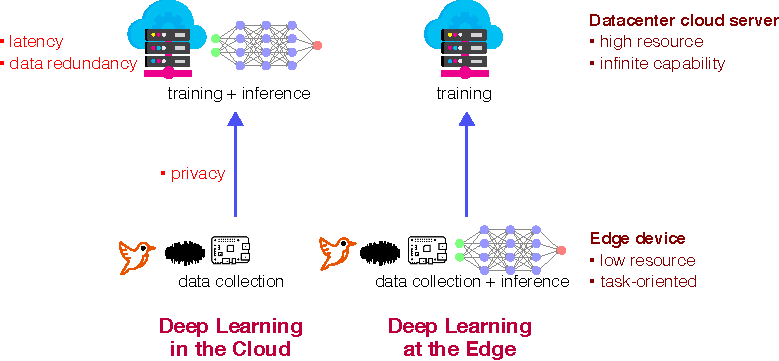
\includegraphics[width=.8\textwidth]{edgeinference}
	\caption{Cloud inference vs edge inference.}
	\label{edgeinference}
\end{figure}

Cloud-based inference utilize servers with high resources and virtual limitless capacity. 
However, cloud-based inference has a number of drawbacks. First, cloud-based inference requires twice the energy compared to local processing. Second is latency. Sending data to the cloud and waiting for result may incur delays which cause real-time applications to fail. Some applications will be totally non-functional if the network is congested or unavailable. Third is privacy as data may leaked during network transfer \citep{Lane2016}. Lastly, cloud-based inference causes scalability issues. Much of the data send to the cloud do not useful information contributing to inefficient network utilization  \cite{Chen2019}.
Fig. \ref{edgeinference} illustrates these differences.

Many applications require only a fixed trained model for inference.
Training the model can be performed offline by at the cloud.
Edge devices perform the necessary inference and send only positive detections to the cloud.

In bioacoustic monitoring, continuous observations is a must to capture rare events.
Storage limitations of PAMs and communication overheads of cloud-based inference impose limitations on continuous real-time monitoring.
Performing inference at the edge and using low-power long-range radio communications such as LoRa seems able to solve the limitations mentioned above \cite{Ayele2018}.

\subsection{Machine Learning Hardware}

This sections lists representative hardware that have been deployed for machine learning at the edge.

\subsubsection{Raspberry Pi}

The Raspberry Pi single board computer (SBC) is the most common devices for edge computing. It can run ML without extra hardware \cite{Xu2018}. The most powerful version is Raspberry Pi 4 running quad-core Cortex-A72 ARM at 1.5 GHz. It can contain up 4GB SDRAM enabling quite a substantial CNN to be implemented. SBCs have the advantage of being easy to used as they run embedded Linux and can be programmed using C, C++ or Python.

\subsubsection{Nvidia Jetson}

The Nvidia Jetson family of devices are programmable hardware containing graphical processing units (GPUs) specially designed to run ML algorithms \cite{Otterness2017}. Each GPU is supervised by an on-board ARM CPU. Three versions are available: TK1, TX1 and TX2. These platforms have high performance but consumes more power and require specialized training to use.

\subsubsection{Intel Movidius}

The Intel Movidius is an  ultra-low-power system-on-chip (SoC) containing hardware specially designed to run ML algorithms. This device as a co-processor and is usually paired with the Raspberry Pi to ML tasks \cite{Andri2017}.

\subsubsection{Field-Programmable Gate Array (FPGA)}

Field-programmable gate arrays are reconfigurable hardware devices that has better power-efficiency than CPUs. At least one study has applied the FPGA for bird recognition \cite{Hervas2017}. The most powerful device for CNNs is the Intel Arria 10 which contains hardware floating-point units \cite{Aydonat2017}. FPGAs commonly embed hardware ARM CPUs to supervise the reconfigurable hardware. FPGAs used to require programming in hardware description languages such as Verilog but frameworks such as OpenCL are faciliting FPGA use among non-hardware designers. Intel and Xilinx supply most of the FPGAs in use today.

\subsubsection{Application-Specific Integrated Circuit (ASIC)}

Application-specific integrated circuits are silicon devices which can implement ML in hardware in the most power-efficient way. They require extensive hardware expertise to design. ASICs have been used for the keyword spotting task \cite{Price2018, Liu2019}.


\FloatBarrier

\subsection{Power-Efficient CNN Inference}

Other than large memory requirements, the other obstacle in implementing deep neural networks in embedded systems high power consumption. Power consumption is directly related to the number of multiply and acummulate operations required. Table \ref{power} lists the power consumption for different operations and sizes of operands.


\begin{table}[h]
\renewcommand{\arraystretch}{1}
\small
\centering
\caption{Energy consumption in multiply-accumulations at 45nm feature size \cite{Horowitz2014}.}
\label{power}
\begin{tabular}{lcccccc}
\toprule
\textbf{Operation} & \textbf{MUL} & \textbf{ADD} \\
\midrule
8-bit integer       &0.2pJ  &0.03pJ \\
32-bit integer      &3.1pJ  &0.1pJ \\
16-bit floating-point&1.1pJ &0.4pJ \\
32-bit floating-point&3.7pJ &0.9pJ\\
\bottomrule
\end{tabular}
\end{table}


\subsubsection{Small CNNs}

One approach to power efficiency is to build CNNs knowing the effects of design decision on power.
In the SqueezeNext model, power is reduced by removing operations that do not contribute to accuracy \cite{Gholami2018}. SqueezeNeXt design variations are more 2x faster and power efficient than the already small MobileNet.


A more popular approach to power efficiency is to build CNNs with just enough complexity to match the application at hand. Table \ref{customcnn} lists CNNs that work with spectrograms. They do not use the typical square image shape used by ImageNet-class CNNs. Instead, the inputs are elongated to match the shape of spectrograms.



\begin{table}[H]
\renewcommand{\arraystretch}{1}
\small
\centering
\caption{Custom CNN for sound recognition.}
\label{customcnn}
\begin{tabular}{lcccccc}
\toprule
\textbf{Study} & \textbf{Layers} & \textbf{Input} & \textbf{Target} & \textbf{Performance} \\
\midrule
Piczak et al \cite{Piczak2015} & 4 (2 CNN, 2 FC) & $1024\times 60$ & Environmental sound & 73.7\% \\
Grill et al \cite{Grill2017} & 7 (4 CNN, 3 FC) & $1000\times 80$ & 1 bird & AUC 87.0\% \\
Meyer et al \cite{Meyer2017} & 7 (all CNN) & $400\times 64$ & Sound events & 86.0\% \\
Mac Aodha \cite{MacAodha2018} & 4 (3 CNN, 1 FC) & $130\times 20$  & Bats & Precision 89.5\% \\
Ozer \cite{Ozer2018} & 7 (5 CNN, 2 FC) & $513\times 93$ & Sound events & 97.4\% \\
Ruff \cite{Ruff2019} & 6 (4 CNN, 2 FC) & $500\times 129$ & 7 owl species & 92.5\% \\
\bottomrule
\end{tabular}
\end{table}

%\FloatBarrier

\subsubsection{Binarized Neural Networks}

Binarized neural networks (BNNs) are deep neural networks that use binarized weights and activations, rather than full precision values \cite{Courbariaux2015}.
They are less accurate than full precision networks but they are closing the accuracy gap (Fig. \ref{bnn-challenge}).
BNNs achieve low power due to much reduced logic switching.
Fig. \ref{bnn-advantage} compares standard convolution with BNNs.


\begin{figure}[H]
    \centering
    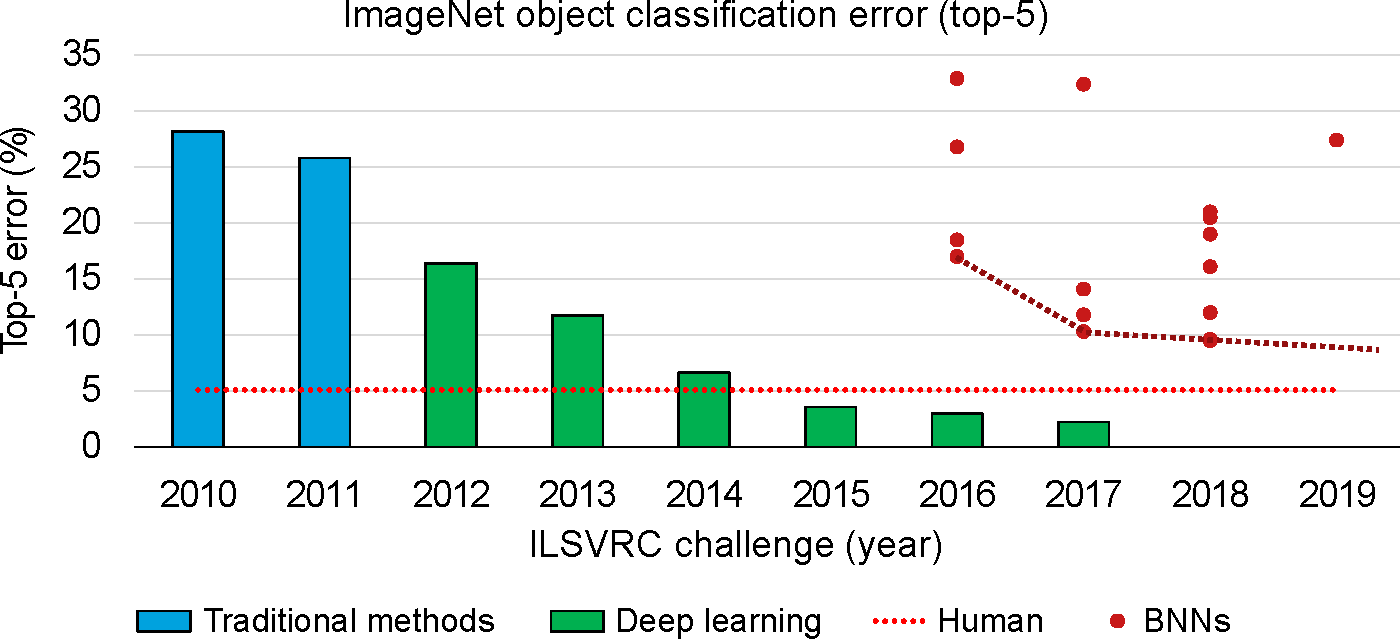
\includegraphics[width=.7\textwidth]{bnn-challenge}
    \caption{BNN still have some catching up to regular CNNs \citep{Rastegari2016}.}
    \label{bnn-challenge}
\end{figure}



%\cite{Pellegrini2017}
\begin{figure}[h]
    \centering
    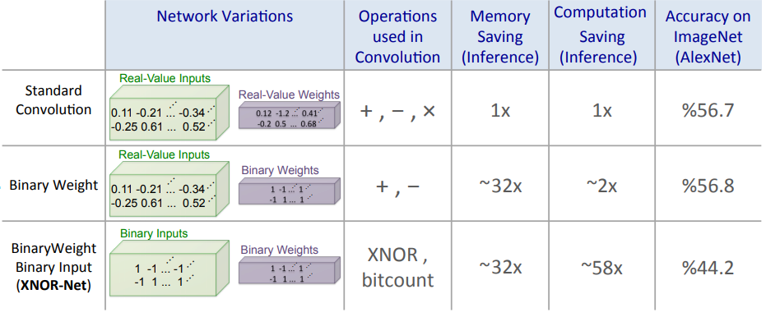
\includegraphics[width=.9\textwidth]{bnn-advantage}
    \caption{Comparison of standard convolution, binary weight/standard input and binary weight/binary input \citep{Rastegari2016}.}
    \label{bnn-advantage}
\end{figure}

BNNs achieve the best efficiency when implemented on FPGA and ASIC. These target devices can be specified to use any operand size leaving no redundant bits. Additionally, multiply and add operations can be replaced with XNOR and population count operations, respectively, substantially reducing the amount of logic circuit.  See Fig. \ref{bnn-popcount}.

\begin{figure}[h]
    \centering
    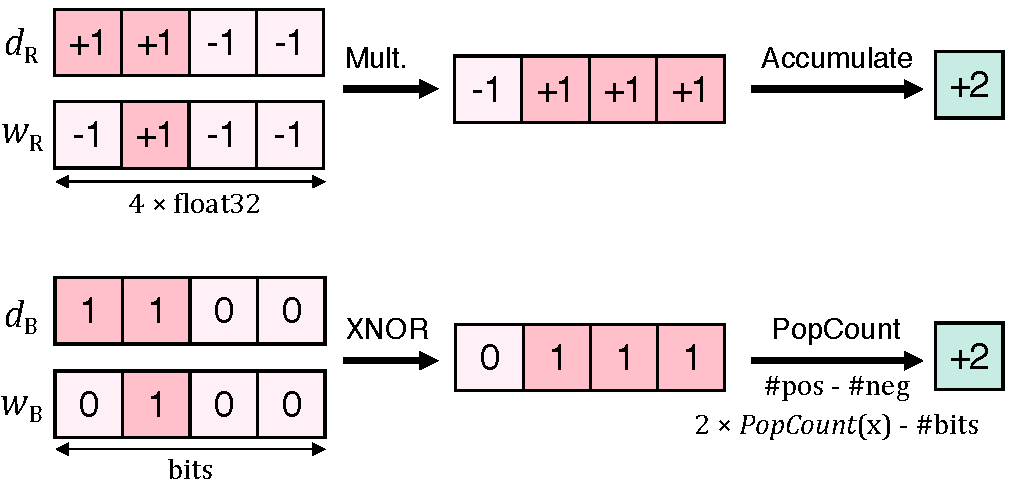
\includegraphics[width=.5\textwidth]{bnn-popcount}
    \caption{Acceleration of binarized neural network by replacing multiply and acummulate operators with XNOR and population count operators, respectively \citep{Rastegari2016}.}
    \label{bnn-popcount}
\end{figure}

\FloatBarrier

\subsubsection{Cascade Classifiers}

Power consumption can be reduced by turning off unnecessary circuits until needed.
Cascade classifiers implement this idea using two classifiers back-to-back.
The first classifier is a `weak' binary classifier which does not have to be very accurate.
A  positive detection activates the second classifier to perform the full multi-class identification.


\begin{figure}[H]
\centering
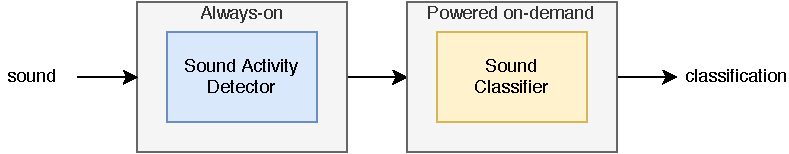
\includegraphics[width=.8\textwidth]{two-stage-classifier-gray}
\caption{Cascade audio classifier.}
\label{two-stage-classifier-gray}
\end{figure}

On the iPhone implementation of the cascade classifier, an always-on processor (AOP) listens to the phrase ``Hey, Siri''.
When the wake-up word is detected, the AOP wakes up the mobile phone enabling more complex speech recognition tasks which require sending voice signals to the cloud \cite{Sigtia2018}.
For the simpler keyword spotting application, the cascade architecture has been implemented on digital signal processor (DSP) \citep{Gruenstein2017} and ASIC \cite{Price2018, Yin2018}.
This architecture has so far not yet applied for bird recognition.
		


\section{Conclusion}

This chapter establishes the context of the research topic.
The importance of automated bird recognition by acoustic methods is outlined.
For bird recognition to be effective on edge devices, it is proposed that a cascade classifier can achieve good performance at low power consumption.
This is the direction taken in the methodology chapter. 

\chapter{Methodology}

This chapter presents the approach used for this research.
 Fig. \ref{phd-methodology} summarizes the steps.

\begin{figure}[h]
\centering
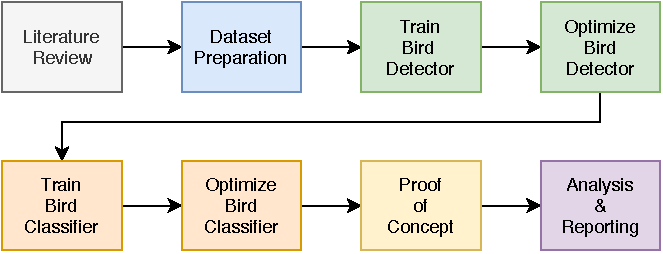
\includegraphics[width=.8\textwidth]{phd-methodology}
\caption{Research methodology.}
\label{phd-methodology}
\end{figure}

\begin{enumerate}
\item To develop 20-species classifier.
\item The number 20 comes from the list of Malaysian Garden birds
\item N shall run 8-bit integer input and parameters
\item Proof on Concept to be run on Raspberry Pi single board computer
\item Raspberry Pi can run acoustic event recognition faster than real time for some large neural networks \citep{Ebbers2018}
\end{enumerate}

 Fig. \ref{cascade-dataflow} summarizes the data flow.


\begin{figure}[H]
\centering
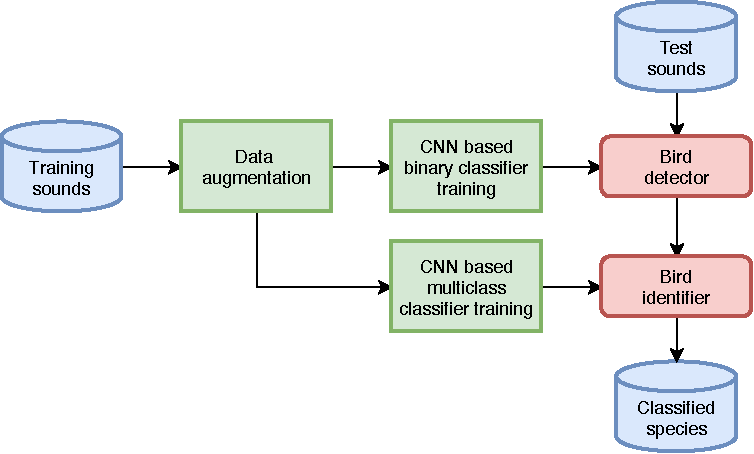
\includegraphics[width=.8\textwidth]{cascade-dataflow}
\caption{Data flow in proposed cascade bird classifier.}
\label{cascade-dataflow}
\end{figure}

\section{Dataset}

 Bird sound dataset not readily usable for deep learning training.
Long sound files to be segmented to 1s clipped, resampled to 8kHz.

\begin{table}[h]
    \centering
    \small
    \caption{Some common bird sound databases.}
	\begin{tabular}{ll}
	\toprule
	\textbf{Dataset} & \textbf{URL} \\
	\midrule
	Xeno-canto & http://xeno-canto.org \\
	Macaulay Library & https://www3.macaulaylibrary.org/browse/taxa/aves \\
	DCASE & http://dcase.community/challenge2018/task-bird-audio-detection \\
	British Birdsong Dataset & https://www.kaggle.com/rtatman/british-birdsong-dataset \\
	LifeCLEF 2018 Bird & https://www.crowdai.org/challenges/lifeclef-2018-bird-monophone \\
	\bottomrule
	\end{tabular}
\end{table}	
	


\section{Bird Detector}


\begin{itemize}
	\item Binary Classifier: Bird/No-bird
	\item Always on: must be simple
	\item When this module detects a possible bird sound, 
			it passes the data to the bird species classifier
	\item Algorithm for this module are based on:
	\begin{itemize}
		\item Voice activity detection for speech recognition
		\item Sound event detection for security
	\end{itemize}
	\item This module must be accurate enough (high TP+FP). FP are taken care by the next module.
\end{itemize}


The bird detector performs the initial detection.
It is as simple as possible as it must run continuously.
The proposed architecture is based on the binarized convolutional neural network (BNN) proposed by \cite{Courbariaux2016}.

	\begin{itemize}
		\item
		The sound detector must listen to continuously streaming audio, ignoring nearly all of it, yet still triggering correctly and instantly.
%		\item
%		On a mobile device, this is particularly challenging when considering that typical mobile devices (e.g. smartphones) have batteries with capacities between 1,000mAh and 2,400mAh
		\item
		Entire system should consume < 1mA to consume < 1\% of the battery per day. \citep{Gruenstein2017}
	\end{itemize}

\begin{figure}
    \centering
    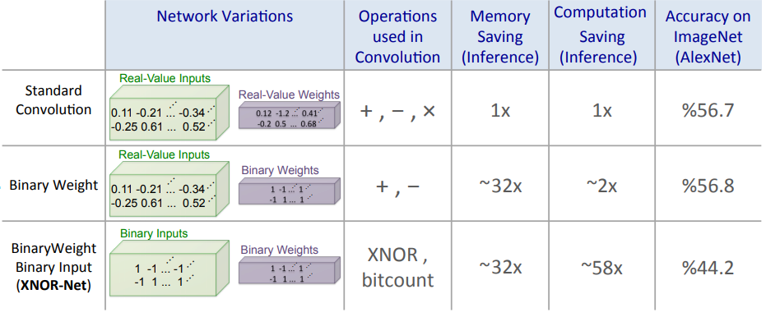
\includegraphics[width=.8\textwidth]{bnn-advantage}
    \caption{Comparison of standard convolution, binary weight/standard input and binary weight/binary input \citep{Rastegari2016}.}
    \label{bnn-advantage}
\end{figure}

\begin{figure}
    \centering
    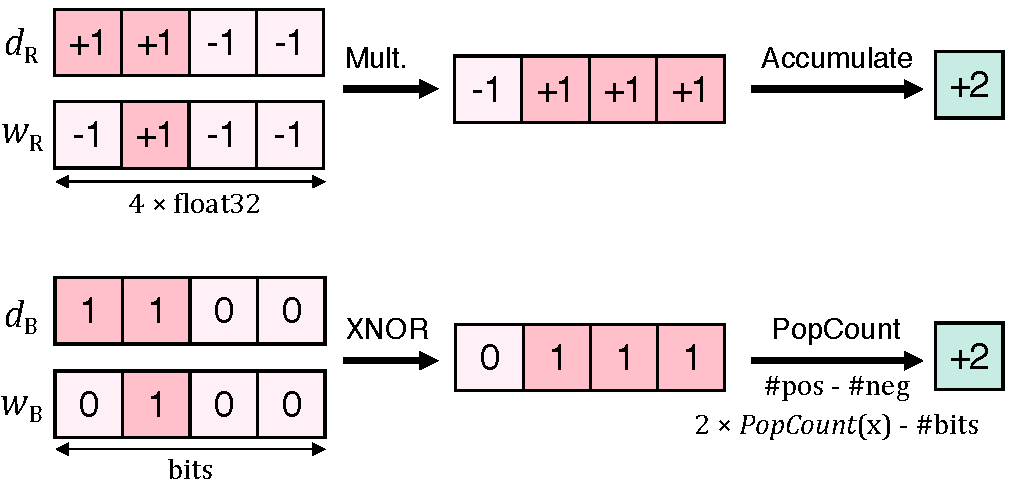
\includegraphics[width=.6\textwidth]{bnn-popcount}
    \caption{Acceleration of binarized neural network by replacing multiply and acummulate operators with XNOR and population count operators, respectively \citep{Rastegari2016}.}
    \label{bnn-popcount}
\end{figure}


\begin{figure}
    \centering
    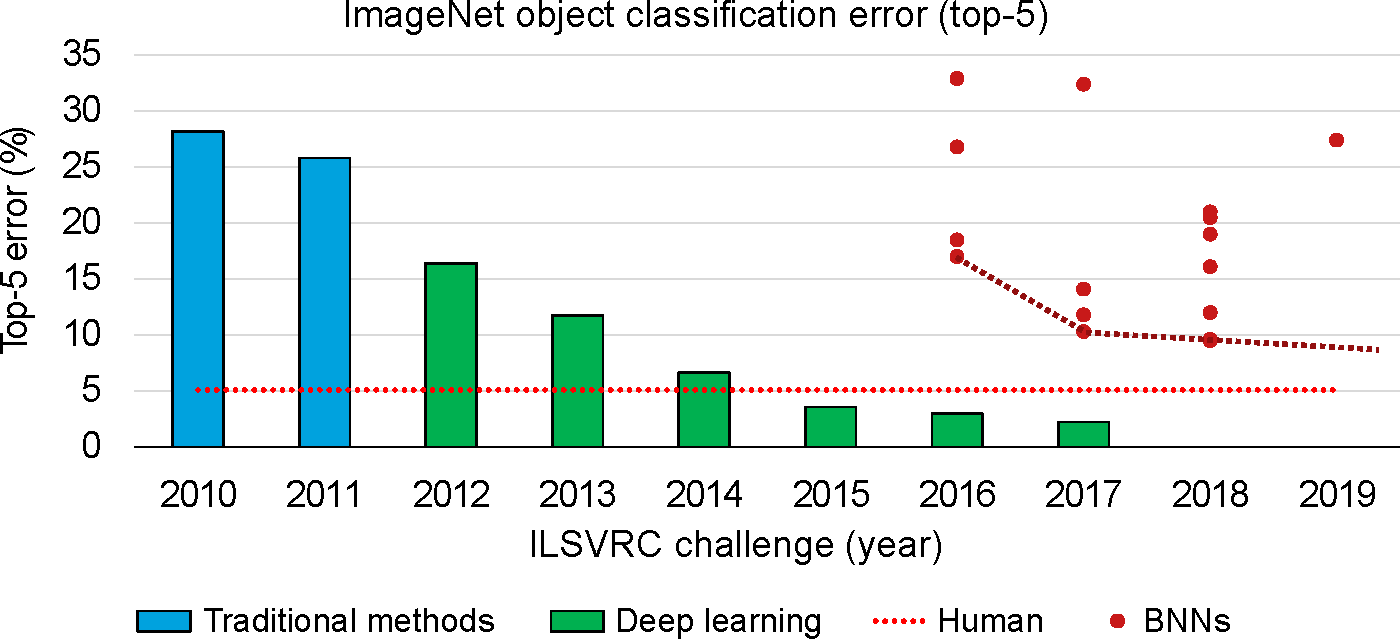
\includegraphics[width=.8\textwidth]{bnn-challenge}
    \caption{BNN still have some catching up to regular CNNs \citep{Rastegari2016}.}
    \label{bnn-challenge}
\end{figure}
\section{Bird Classifier}

 The classifier algorithm has to be lightweight to fit the embedded platform
 Popular CNN does not match the input image square vs elongated
 Use of an existing DNN model as a base, 
			then modified to find the best parameters for bird sound.

\begin{table} 
    \small
    \centering
    \caption{Hand-crafted CNN for bird recognition.}
    \begin{tabular}{lrrrrrrr}%{.15\textwidth}p{.4\textwidth}p{.35\textwidth}}
    \toprule
    \textbf{Reference} & 
    \textbf{DNN } &
    \textbf{layers} &
    \textbf{param.} &
    \textbf{MAC} &
    \textbf{acc.} \\
    \midrule
    \cite{Takahashi2016} & - & 9 & 257M & ? & 92.8 \% \\
    \cite{Grill2017} & bulbul & 8 & ? & ? & ?\\
    \cite{Grill2017} & sparrow & 10 &  ? & ? & ?\\
    \cite{Meyer2017} & custom x 3 & 8 & 233-452 M & 1239-2655 M & 80.3-86.0 \% \\
    \cite{Ruff2019} & custom & 6 & - & - & 63.1-92.5\% \\ %500x129 res, 7 species
    \bottomrule
    \end{tabular}
\end{table}

\subsection{STFT)}

\subsection{Gammatone)}

\subsection{CQT Spectrogram)}

\begin{figure}[H]
\centering
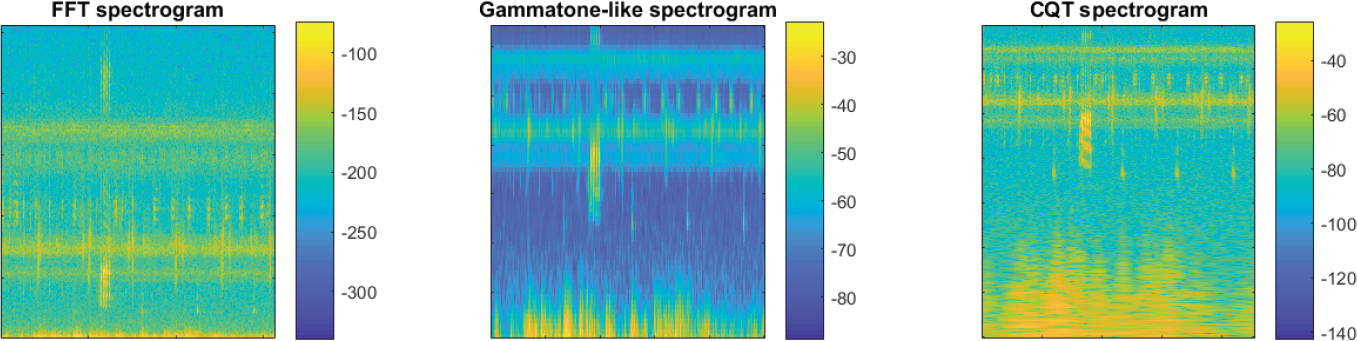
\includegraphics[width=.8\textwidth]{fft-gfcc-cqt}
\caption{STFT, Gammatone and CQT spectrograms \citep{Xie2017}.}
\end{figure}

\FloatBarrier

\subsection{Spectral Image Features (SIF)}

\begin{figure}[h]
\centering
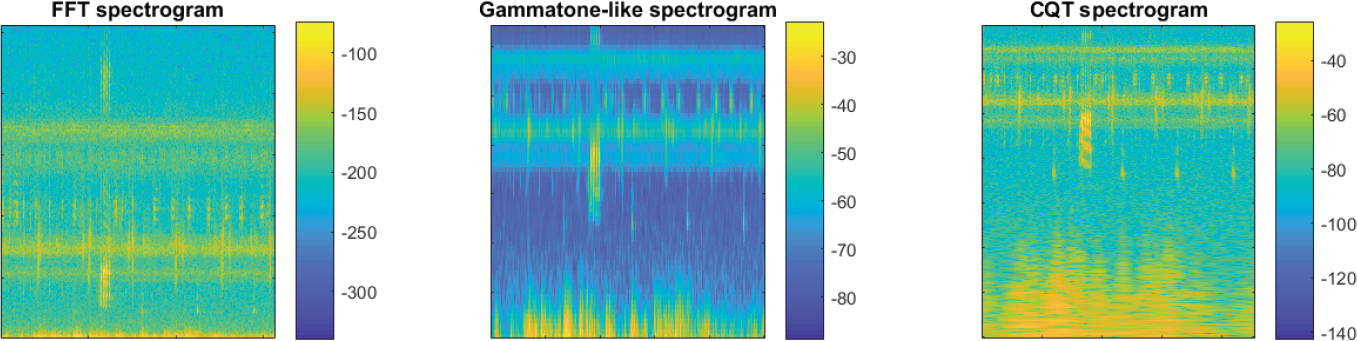
\includegraphics[width=.8\textwidth]{fft-gfcc-cqt}
\caption{STFT, Gammatone and CQT spectrograms \citep{Xie2017}.}
\end{figure}


Detect the bird vocalizations using \cite{Fodor2013}, \cite{Lasseck2015} and \cite{Potamitis2015}.



\section{Training process}

The downloaded sound files will be used to train the networks under consideration.

\section{Evaluation}


To evaluate the performance of each model, we employ the following metrics:

\subsubsection{Precision}

This metric is defined as the proportion of true positives that are correctly identified by the detector. 
This metric is calculated by taking into account the True Positives (TP) and False Negatives (FN):

\[
\mathrm{Precision} = P = \frac{TP}{TP + FN}
\]

\subsubsection{Accuracy}

\[
\mathrm{Accuracy} = \frac{TP+TN}{\mathrm{total}}
\]


\par{\textit{Inferences-per-second (IPS)}}: the rate at which the bird classifier is capable of processing bird vocalizations

\subsubsection{Computational complexity}


\subsubsection{Power consumption}

 

\chapter{Conclusion}

What is different?

\begin{itemize}
\item Not using ImageNet-class CNN which are too big
\item Cascade classifier to improve accuracy and power consumption
\item Binary first-stage classifier to minimize static power
\item Small lightweight CNN second-stage with just enough features
\item Application of spectral image features (SIF)
\item Measurement of power to compute each inference
\item Mapping of classifier to platform
\item Platform recommendations
\item Possible additional work: FFT-based audio compression and IoT proof-of-concept (RasPi and Portenta)
\end{itemize} 
%
\chapter{Conclusion}

What is different?

\begin{itemize}
\item Not using ImageNet-class CNN which are too big
\item Cascade classifier to improve accuracy and power consumption
\item Binary first-stage classifier to minimize static power
\item Small lightweight CNN second-stage with just enough features
\item Application of spectral image features (SIF)
\item Measurement of power to compute each inference
\item Mapping of classifier to platform
\item Platform recommendations
\item Possible additional work: FFT-based audio compression and IoT proof-of-concept (RasPi and Portenta)
\end{itemize} 
 
%----------------------------------------------------------------------------------------
%	APPENDICES
%----------------------------------------------------------------------------------------

%\addtocontents{toc}{\vspace{2em}} % Add a gap in the Contents, for aesthetics
%\appendix % Starts of appendices

%\numberedchapter
%

\chapter{About Appendices} \label{appA}


Appendices are optional and should only be used if necessary.
%\input{MainText/appendixB}
%\input{MainText/appendixC}

%----------------------------------------------------------------------------------------
%	BIBLIOGRAPHY
%----------------------------------------------------------------------------------------

\addtocontents{toc}{\vspace{2em}} % Add a gap in the Contents, for aesthetics
\unnumberedchapter{References} % Title of the unnumbered chapter
%\bibliography{references} % 
\renewcommand*{\bibfont}{\small}
\renewcommand{\bibname}{References}
\printbibliography
\end{document}  